\documentclass{standalone}
\usepackage{tikz}
\begin{document}
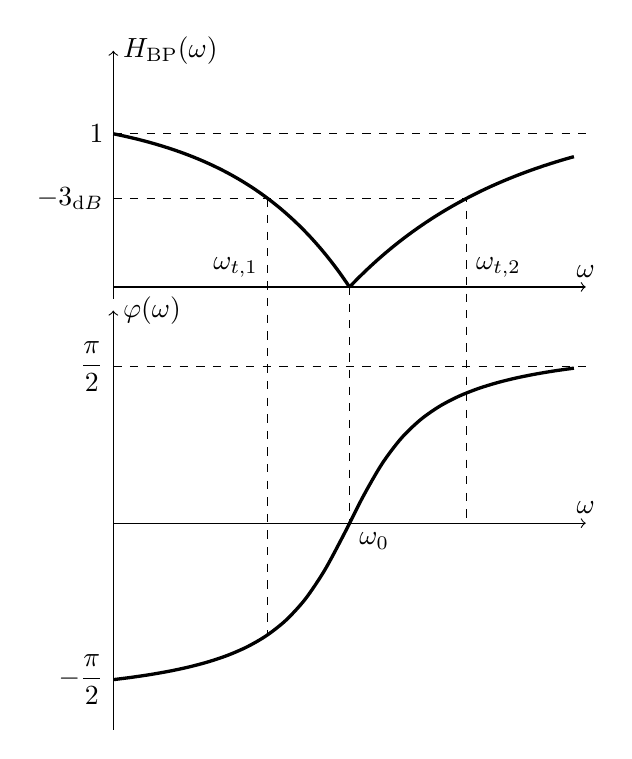
\begin{tikzpicture}[scale=1.5]
    \draw[->](0,1.9)--(0,4)node[right]{$H_{\mathrm{BP}}(\omega)$};
    \draw[->](0,2)--(4,2)node[above]{$\omega$};
    \draw[very thick,smooth, domain=0:2]plot(\x,{-1.5*e^(\x-2)+3.5});
    \draw[very thick,smooth, domain=2:3.9]plot(\x,{-1.5*e^(0.7*(-\x+2))+3.5});
    \draw[->](0,-1.75)--(0,1.8)node[right]{$\varphi(\omega)$};
    \draw[->](0,0)--(4,0)node[above]{$\omega$};
    \draw[very thick, smooth, domain=0:3.9]plot(\x,{pi/180*atan(2*\x-4)});
    \draw[dashed](0,3.297)node[left]{$1$}--(4,3.297);
    \draw[dashed](2,2)--(2,0)node[below right]{$\omega_0$};
    \draw[dashed](0,1.326)node[left]{$\displaystyle\frac{\pi}{2}$}--(4,1.326);
    \node[left]at(0,-1.326){$-\displaystyle\frac{\pi}{2}$};
    \draw[dashed](0,2.75)node[left]{$-3_{\mathrm{d}B}$}--(1.307,2.75)--(2.99,2.75)--(2.99,2)node[above right]{$\omega_{t,2}$}--(2.99,0);
    \draw[dashed](1.307,2.75)--(1.307,2)node[above left]{$\omega_{t,1}$}--(1.307,-0.946);
\end{tikzpicture}
\end{document}